\section{Non-Linear Filters}

Non-linear filtering is set of operations that is performed on a neighbourhood of pixels in a digital image. In linear filtering the sum of an image's responses to two or more filters is the same as the sum of those filters applied to the image once. This is not the case in non-linear filtering, however there are scenarios where a non-linear filter can achieve superior results. A non-linear filter's application to an image is not simply it's convolution with that image.

\subsubsection{The Median Filter}

The median filter is useful for denoising an image, much like the linear box and Gaussian filters (section \ref{subsection:kernels}). A median filter's applications returns the median valued pixel found in the neighbourhood under its mask. This is a more complex operation than to convolve one signal with another however it can be computed in linear time \cite{cormen_2001}. It is superior to the Gaussian filter at denoising images, particularly where intensities vary largely, which would skew the weighted average of a linear filter. In Figure \ref{fig:shot_noise} the median filter demonstrates a superior ability to remove salt and pepper noise as compared to the Gaussian filter.

\begin{figure*}[htbp]
    \centering 
    \begin{subfigure}[b]{0.3\textwidth}
        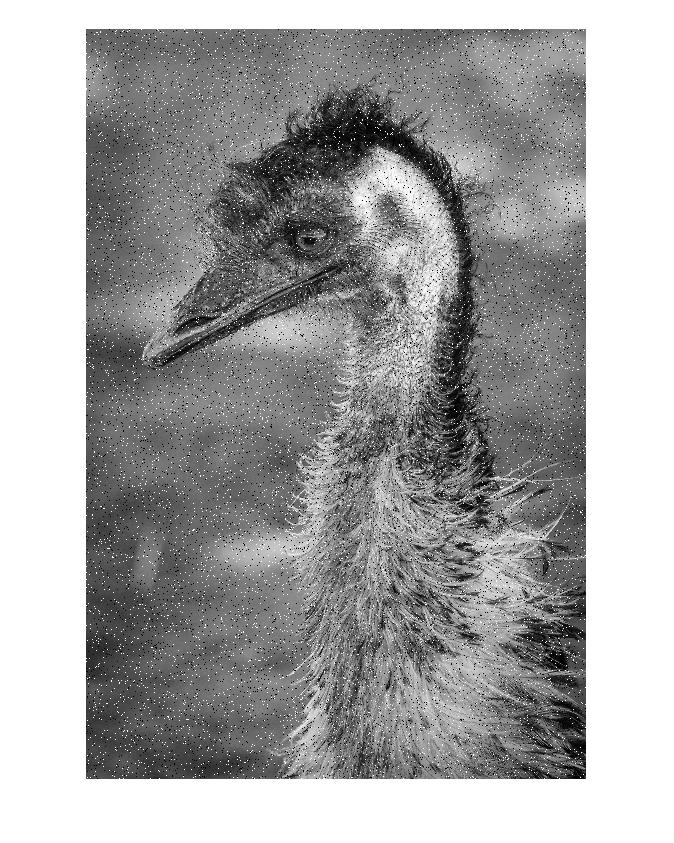
\includegraphics[width=\textwidth]{emu_noise}
        \caption{Salt and Pepper Noise}
        \label{fig:emu_noise}
    \end{subfigure}
    \begin{subfigure}[b]{0.3\textwidth}
        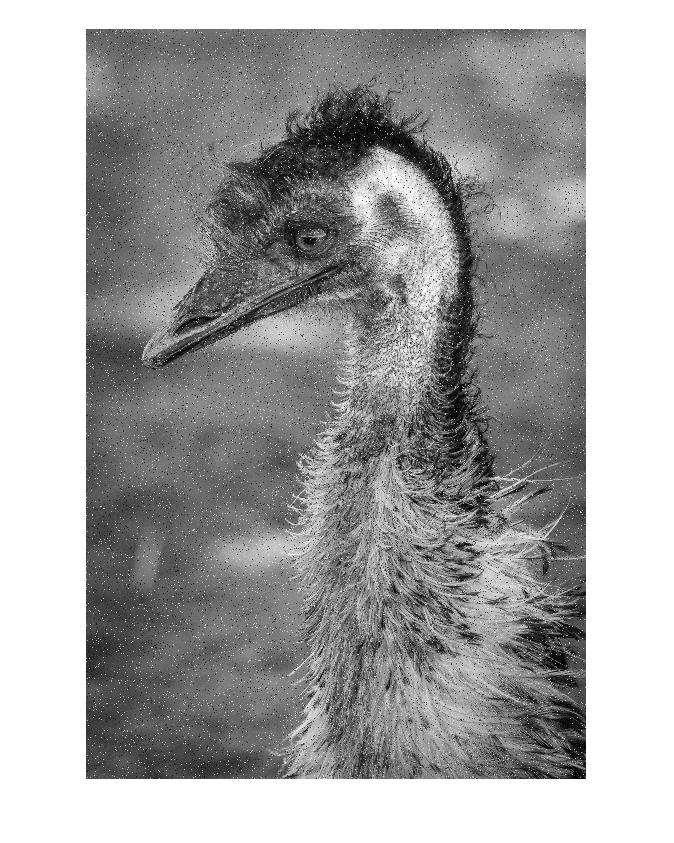
\includegraphics[width=\textwidth]{emu_gauss}
        \caption{7x7 Gaussian}
        \label{fig:emu_gauss}
    \end{subfigure}
    \begin{subfigure}[b]{0.3\textwidth}
        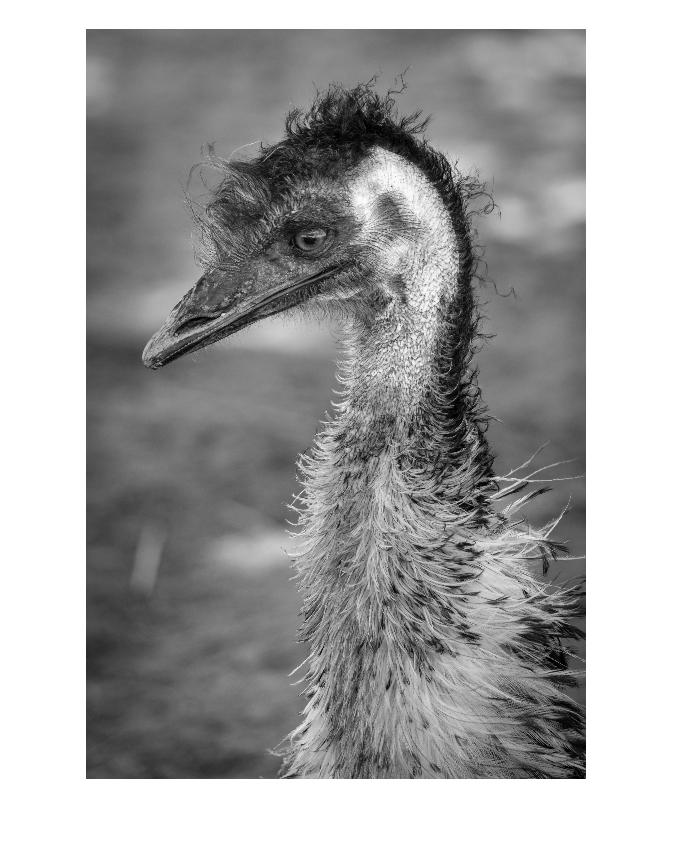
\includegraphics[width=\textwidth]{emu_median}
        \caption{7x7 Median Filter}
        \label{fig:emu_median}
    \end{subfigure}
    \captionsetup{format=hang}
    \caption{Filtering out salt and pepper noise with Gaussian and median filter. Original image by Grant Durr.}
    \label{fig:shot_noise}
\end{figure*}